%
% firmware.tex
%
% Copyright (C) 2022 by SpaceLab.
%
% TTC 2.0 Module
%
% This work is licensed under the Creative Commons Attribution-ShareAlike 4.0
% International License. To view a copy of this license,
% visit http://creativecommons.org/licenses/by-sa/4.0/.
%

%
% \brief Firmware project slides.
%
% \author Gabriel Mariano Marcelino <gabriel.mm8@gmail.com>
% \author Miguel Boing <miguelboing13@gmail.com>
%
% \version 0.1.0
%
% \date 2022/07/28
%


\begin{frame}{Overview}

    \begin{columns}[t]
        \begin{column}[t]{0.6\textwidth}
            \begin{itemize}
                \vspace{1cm}
                \item Language: C
                \vspace{0.5cm}
                \item OS: FreeRTOS v10.2.1
            \end{itemize}
        \end{column}
        \begin{column}[t]{0.4\textwidth}
            \begin{figure}[!ht]
                \begin{center}
                    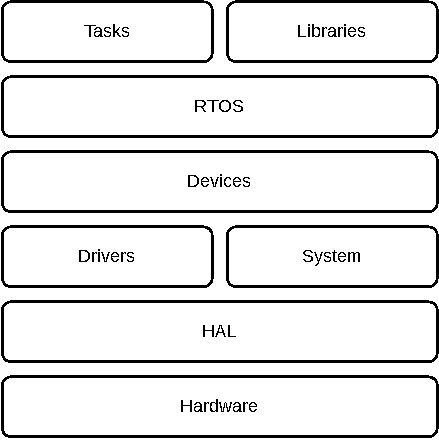
\includegraphics[width=4cm]{figures/ttc2-layers.pdf}
                \end{center}
            \end{figure}
        \end{column}
    \end{columns}

\end{frame}

% #########################################################################
% #########################################################################

\begin{frame}{System Tasks}

\begin{table}[!h]\scriptsize
    \centering
    \label{tab:firmware-tasks}
    \begin{tabular}{lccccc}
        \toprule[1.5pt]
        \textbf{Name}          & \textbf{Priority} & \textbf{Initial delay [ms]} & \textbf{Period [ms]} & \textbf{Stack [bytes]} \\
        \midrule
        Command Processing     & Highest & 0     & 100       & 500 \\
        Heartbeat              & Lowest  & 0     & 500       & 160 \\
        Housekeeping           & Medium  & 2000  & 10000     & 160 \\
        Radio Reset            & High    & 60000 & 60000     & 128 \\
        Startup                & Medium  & 0     & Aperiodic & 128 \\
        System Reset           & Medium  & 0     & 36000000  & 128 \\
        Time Control           & Medium  & 1000  & 1000      & 128 \\
        Uplink                 & Highest & 2000  & 500       & 500 \\
        Watchdog Reset         & Lowest  & 0     & 100       & 150 \\
        \bottomrule[1.5pt]
    \end{tabular}
\end{table}

\end{frame}

\begin{frame}{System Tasks}

    \begin{itemize}
        \item \textbf{Command Processing}: Process incomming commands (physical interfaces).
        \item \textbf{Heartbeat}: Blinks a status LED at a rate of 1 Hz.
        \item \textbf{Housekeeping}: This task manages the general operation of
the TTC.
        \item \textbf{Radio Reset}: Resets the radio at 600 seconds.
        \item \textbf{Startup}: Initializes the TTC 2.0 module.
        \item \textbf{System Reset}: Resets the microcontroller by software at every 10 hours.
        \item \textbf{Time Control}: Manages the system time.
        \item \textbf{Uplink}: Monitors radio for upcoming packages and stores it in memory.
        \item \textbf{Watchdog Reset}: Resets the watchdog timers at every 100 miliseconds.
    \end{itemize}

 \end{frame}


% #########################################################################
% #########################################################################

\begin{frame}{System Parameters}

\begin{table}[!htb]\tiny
    \centering
    \label{tab:vars-and-pars}
    \begin{tabular}{cll}
        \toprule[1.5pt]
        \textbf{ID} & \textbf{Name/Description} & \textbf{Type}\\
        \midrule
        0   & Device ID (0xCC2A or 0xCC2B)                                      & uint16 \\
        1   & Hardware version                                                  & uint8 \\
        2   & Firmware version (ex.: ``v1.2.3''' = 0x00010203)                  & uint32 \\
        3   & Time counter in millseconds                                       & uint32 \\
        4   & Reset counter                                                     & uint16 \\
        5   & Last reset cause:                                                 & uint8 \\
        6   & Input voltage of the $\mu$C in mV                                 & uint16 \\
        7   & Input current of the $\mu$C in mA                                 & uint16 \\
        8   & Temperature of the $\mu$C in K                                    & uint16 \\
        9   & Input voltage of the radio in mV                                  & uint16 \\
        10  & Input current of the radio in mA                                  & uint16 \\
        11  & Temperature of the radio in K                                     & uint16 \\
        12  & Last valid command (uplink packet ID)                             & uint8 \\
        13  & RSSI of the last valid telecommand                                & uint16 \\
        14  & Temperature of the antenna module in K                            & uint16 \\
        15  & Antenna module status bits                                        & uint16 \\
        16  & Antenna deployment status                                         & uint8 \\
        17  & Antenna deployment hibernation                                    & uint8 \\
        18  & TX enable                                                         & uint8 \\
        19  & TX packet counter                                                 & uint32 \\
        20  & RX packet counter (valid packets)                                 & uint32 \\
        21  & TX packets available in the FIFO buffer                           & uint8 \\
        22  & RX packets available in the FIFO buffer                           & uint8 \\
        23  & Number of bytes of the first available packet in the RX buffer    & uint16 \\
        \bottomrule[1.5pt]
    \end{tabular}
\end{table}

\end{frame}

\begin{frame}{Commands}

\begin{table}[!htb]\scriptsize
    \centering
    \label{tab:vars-and-pars}
    \begin{tabular}{cll}
        \toprule[1.5pt]
        \textbf{ID} & \textbf{Command} & \textbf{Parameters}\\
        \midrule
        1   & Read parameter              & Parameter ID \\
        2   & Write parameter             & Parameter ID + Parameter value \\
        3   & Transmit packet             & Data to transmit (payload of the NGHam packet) \\
        4   & Read first available packet & None \\
        \bottomrule[1.5pt]
    \end{tabular}
\end{table}

\end{frame}

% #########################################################################
% #########################################################################

\begin{frame}{Development Environment}

    \begin{columns}[t]
        \begin{column}[t]{0.6\textwidth}
            \begin{itemize}
                \vspace{0.4cm}
                \item Hardware: Engineering Model (EM)
                \vspace{0.4cm}
                \item Programmer: Texas Instruments MSP-FET programmer
                \vspace{0.4cm}
                \item IDE/Compiler: Code Composer Studio
                \vspace{0.4cm}
            \end{itemize}
        \end{column}
        \begin{column}[t]{0.5\textwidth}
            \vspace{1cm}
            \begin{figure}[!ht]
                \begin{center}
                    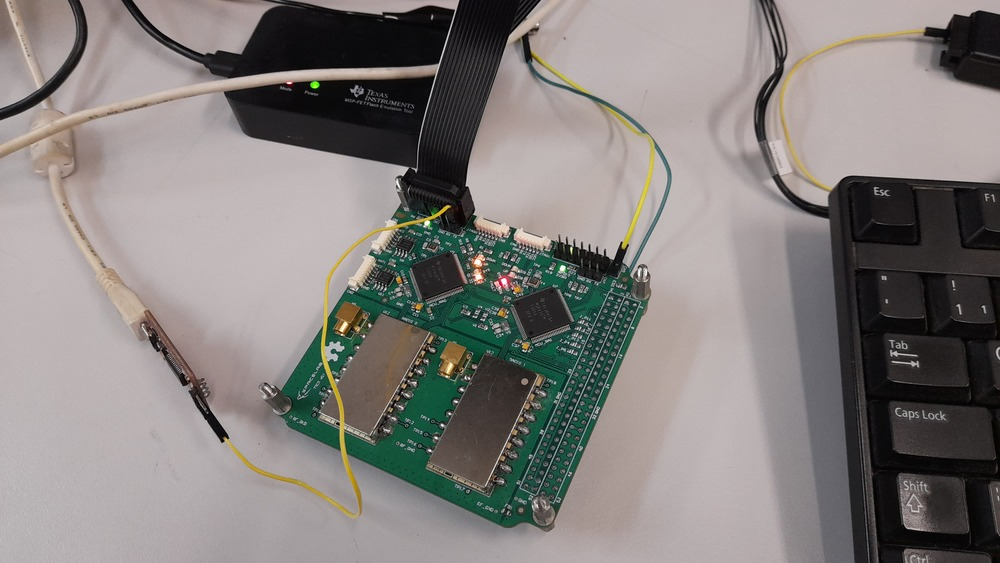
\includegraphics[width=5cm]{figures/ttc2-bench.jpg}
                \end{center}
            \end{figure}
        \end{column}
    \end{columns}

\end{frame}

% #########################################################################
% #########################################################################

\begin{frame}{Verification \& Validation}

    \begin{itemize}
        \item Unit tests framework: \href{https://cmocka.org/}{\textcolor{blue}{\underline{CMocka}}}
        \vspace{0.5cm}
        \item Static analysis tool: \href{https://cppcheck.sourceforge.io/}{\textcolor{blue}{\underline{CppCheck}}}
        \vspace{0.5cm}
        \item Code style standard: \href{https://www.misra.org.uk/}{\textcolor{blue}{\underline{MISRA-C 2012}}}
    \end{itemize}

\end{frame}

\begin{frame}{Verification \& Validation: TDD Flow}

    \begin{figure}[!ht]
        \begin{center}
            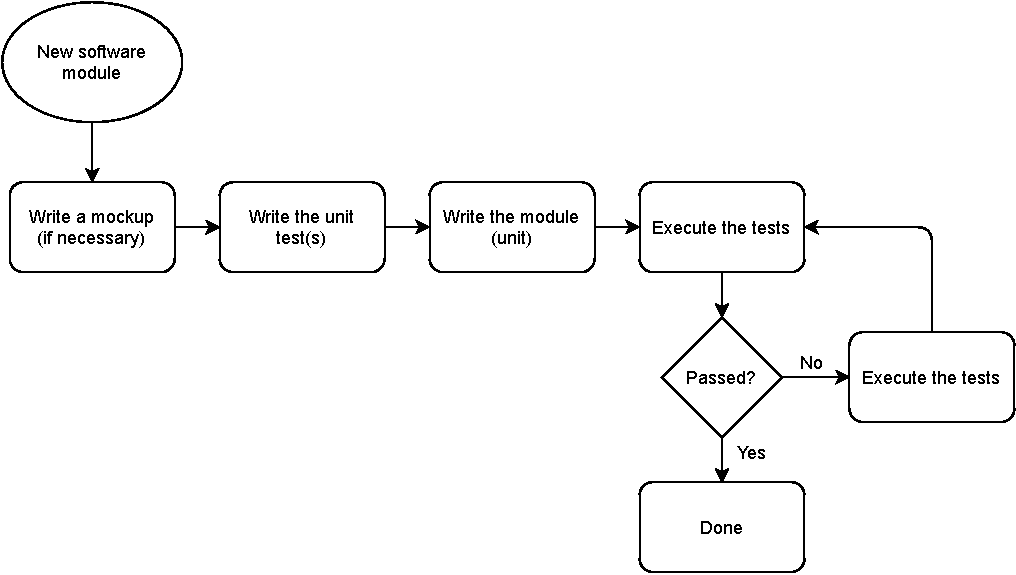
\includegraphics[width=11cm]{figures/tdd-flow.pdf}
        \end{center}
    \end{figure}

\end{frame}

\begin{frame}{Verification \& Validation: Development Flow}

    \begin{figure}[!ht]
        \begin{center}
            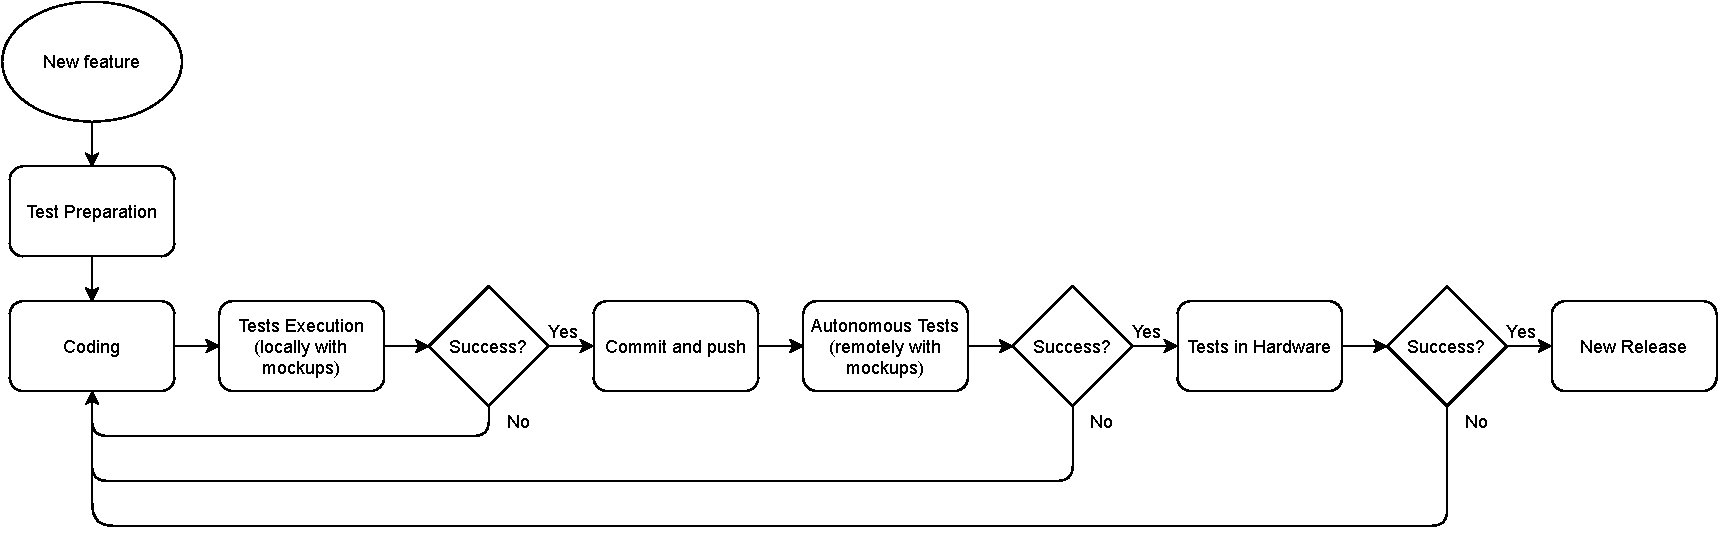
\includegraphics[width=11cm]{figures/dev-flow.pdf}
        \end{center}
    \end{figure}

\end{frame}